\section{Diodo}

Un diodo es un componente electrónico de dos terminales que permite la circulación de la corriente eléctrica a través de él en un solo sentido.1​ Este término generalmente se usa para referirse al diodo semiconductor, el más común en la actualidad; consta de una pieza de cristal semiconductor conectada a dos terminales eléctricos. El diodo de vacío (que actualmente ya no se usa, excepto para tecnologías de alta potencia) es un tubo de vacío con dos electrodos: una lámina como ánodo, y un cátodo.\citep{diodoWiki}\\

De forma simplificada, la curva característica de un diodo (I-V) consta de dos regiones: por debajo de cierta diferencia de potencial, se comporta como un circuito abierto (no conduce), y por encima de ella como un circuito cerrado con una resistencia eléctrica muy pequeña. Debido a este comportamiento, se les suele denominar rectificadores, ya que son dispositivos capaces de suprimir la parte negativa de cualquier señal, como paso inicial para convertir una corriente alterna en corriente continua. Su principio de funcionamiento está basado en los experimentos de Lee De Forest.\citep{diodoWiki}\\


Los primeros diodos eran válvulas o tubos de vacío, también llamados válvulas termoiónicas constituidos por dos electrodos rodeados de vacío en un tubo de cristal, con un aspecto similar al de las lámparas incandescentes. El invento fue desarrollado en 1904 por John Ambrose Fleming, empleado de la empresa Marconi, basándose en observaciones realizadas por Thomas Alva Edison.\citep{diodoWiki}\\


Al igual que las lámparas incandescentes, los tubos de vacío tienen un filamento (el cátodo) a través del cual circula la corriente, calentándolo por efecto Joule. El filamento está tratado con óxido de bario, de modo que al calentarse emite electrones al vacío circundante los cuales son conducidos electrostáticamente hacia una placa, curvada por un muelle doble, cargada positivamente (el ánodo), produciéndose así la conducción. Evidentemente, si el cátodo no se calienta, no podrá ceder electrones. Por esa razón, los circuitos que utilizaban válvulas de vacío requerían un tiempo para que las válvulas se calentaran antes de poder funcionar y las válvulas se quemaban con mucha facilidad.\citep{diodoWiki}\\


\section{Diodo Semiconductor}

\begin{figure}[h!]
\centering
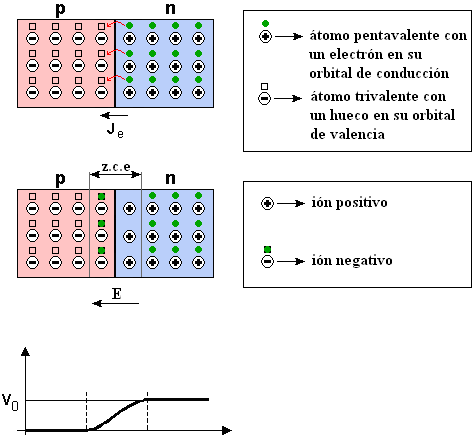
\includegraphics[scale=0.5]{DiodoSem.png}
\caption{Formación de la región de agotamiento, en la gráfica z.c.e.}
\label{fig:diodoSem}
\end{figure}

Un diodo semiconductor moderno está hecho de cristal semiconductor como el silicio con impurezas en él para crear una región que contenga portadores de carga negativa (electrones), llamada semiconductor de tipo n, y una región en el otro lado que contenga portadores de carga positiva (huecos), llamada semiconductor tipo p. Las terminales del diodo se unen a cada región. El límite dentro del cristal de estas dos regiones, llamado una unión PN, es donde la importancia del diodo toma su lugar. El cristal conduce una corriente de electrones del lado n (llamado cátodo), pero no en la dirección opuesta; es decir, cuando una corriente convencional fluye del ánodo al cátodo (opuesto al flujo de los electrones).\citep{diodoWiki}\\

Al unir ambos cristales, se manifiesta una difusión de electrones del cristal n al p (Je). Al establecerse una corriente de difusión, aparecen cargas fijas en una zona a ambos lados de la unión, zona que recibe el nombre de región de agotamiento.\citep{diodoWiki}\\

A medida que progresa el proceso de difusión, la región de agotamiento va incrementando su anchura profundizando en los cristales a ambos lados de la unión. Sin embargo, la acumulación de iones positivos en la zona n y de iones negativos en la zona p, crea un campo eléctrico (E) que actuará sobre los electrones libres de la zona n con una determinada fuerza de desplazamiento, que se opondrá a la corriente de electrones y terminará deteniéndolos.\citep{diodoWiki}\\

Este campo eléctrico es equivalente a decir que aparece una diferencia de tensión entre las zonas p y n. Esta diferencia de potencial (VD) es de 0,7 V en el caso del silicio y 0,3 V para los cristales de germanio.\citep{diodoWiki}\\

La anchura de la región de agotamiento una vez alcanzado el equilibrio, suele ser del orden de 0,5 micras pero cuando uno de los cristales está mucho más dopado que el otro, la zona de carga espacial es mucho mayor.\citep{diodoWiki}\\

Cuando se somete al diodo a una diferencia de tensión externa, se dice que el diodo está polarizado, pudiendo ser la polarización directa o inversa.\citep{diodoWiki}\\

\section{Polarización directa de un diodo}

\begin{figure}[h!]
\centering
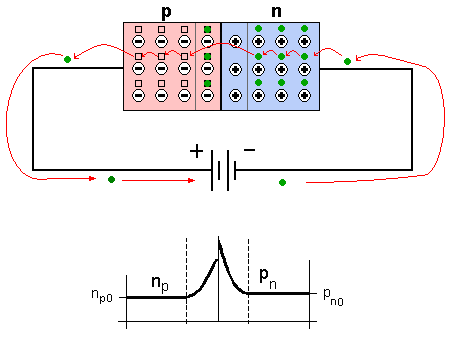
\includegraphics[scale=0.4]{PolDir.png}
\caption{Formación de la región de agotamiento, en la gráfica z.c.e.}
\label{fig:diodoDir}
\end{figure}

En este caso, la batería disminuye la barrera de potencial de la zona de carga espacial, permitiendo el paso de la corriente de electrones a través de la unión; es decir, el diodo polarizado directamente conduce la electricidad.\citep{diodoWiki}\\

Para que un diodo esté polarizado directamente, se debe conectar el polo positivo de la batería al ánodo del diodo y el polo negativo al cátodo. En estas condiciones podemos observar que:\citep{diodoWiki}\\



\begin{itemize}
    \item El polo negativo de la batería repele los electrones libres del cristal n, con lo que estos electrones se dirigen hacia la unión p-n.
    \item El polo positivo de la batería atrae a los electrones de valencia del cristal p, esto es equivalente a decir que empuja a los huecos hacia la unión p-n.
    \item Cuando la diferencia de potencial entre los bornes de la batería es mayor que la diferencia de potencial en la zona de carga espacial, los electrones libres del cristal n, adquieren la energía suficiente para saltar a los huecos del cristal p, los cuales previamente se han desplazado hacia la unión p-n.
    \item Una vez que un electrón libre de la zona n salta a la zona p atravesando la zona de carga espacial, cae en uno de los múltiples huecos de la zona p convirtiéndose en electrón de valencia. Una vez ocurrido esto el electrón es atraído por el polo positivo de la batería y se desplaza de átomo en átomo hasta llegar al final del cristal p, desde el cual se introduce en el hilo conductor y llega hasta la batería.
    \end{itemize}
    
    De este modo, con la batería cediendo electrones libres a la zona n y atrayendo electrones de valencia de la zona p, aparece a través del diodo una corriente eléctrica constante hasta el final.\citep{diodoWiki}\\




\section{Polarización inversa de un diodo}

\begin{figure}[h!]
\centering
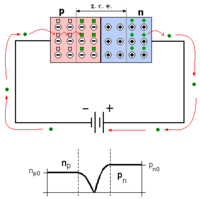
\includegraphics[scale=0.7]{PolInv.png}
\caption{Formación de la región de agotamiento, en la gráfica z.c.e.}
\label{fig:diodoInv}
\end{figure}

En este caso, el polo negativo de la batería se conecta a la zona p y el polo positivo a la zona n, lo que hace aumentar la zona de carga espacial, y la tensión en dicha zona hasta que se alcanza el valor de la tensión de la batería, tal y como se explica a continuación:\citep{diodoWiki}\\


\begin{itemize}
    \item El polo positivo de la batería atrae a los electrones libres de la zona n, los cuales salen del cristal n y se introducen en el conductor dentro del cual se desplazan hasta llegar a la batería. A medida que los electrones libres abandonan la zona n, los átomos pentavalentes que antes eran neutros, al verse desprendidos de su electrón en el orbital de conducción, adquieren estabilidad (8 electrones en la capa de valencia, ver semiconductor y átomo) y una carga eléctrica neta de +1, con lo que se convierten en iones positivos.
    \item El polo negativo de la batería cede electrones libres a los átomos trivalentes de la zona p. Recordemos que estos átomos sólo tienen 3 electrones de valencia, con lo que una vez que han formado los enlaces covalentes con los átomos de silicio, tienen solamente 7 electrones de valencia, siendo el electrón que falta el denominado hueco. El caso es que cuando los electrones libres cedidos por la batería entran en la zona p, caen dentro de estos huecos con lo que los átomos trivalentes adquieren estabilidad (8 electrones en su orbital de valencia) y una carga eléctrica neta de -1, convirtiéndose así en iones negativos.
    \item Este proceso se repite una y otra vez hasta que la zona de carga espacial adquiere el mismo potencial eléctrico que la batería.
    
    
\end{itemize}

En esta situación, el diodo no debería conducir la corriente; sin embargo, debido al efecto de la temperatura se formarán pares electrón-hueco (ver semiconductor) a ambos lados de la unión produciendo una pequeña corriente (del orden de 1 μA) denominada corriente inversa de saturación. Además, existe también una denominada corriente superficial de fugas la cual, como su propio nombre indica, conduce una pequeña corriente por la superficie del diodo; ya que en la superficie, los átomos de silicio no están rodeados de suficientes átomos para realizar los cuatro enlaces covalentes necesarios para obtener estabilidad. Esto hace que los átomos de la superficie del diodo, tanto de la zona n como de la p, tengan huecos en su orbital de valencia con lo que los electrones circulan sin dificultad a través de ellos. No obstante, al igual que la corriente inversa de saturación, la corriente superficial de fuga es usualmente despreciable.\citep{diodoWiki}\\



\bibliographystyle{plain}
\bibliography{references}
\end{document}
